% !Mode:: "TeX:UTF-8"
\section{研究背景及意义}
\subsection{课题研究背景}
\subsubsection{软件定义网络SDN}
%在传统的网络架构中,数据平面和控制平面没有分离,是集成在同一处的硬 件系统上的。这使得新业务在引进时十分不便,一方面需要在路由交换、数据处 理等业务之外进行相关处理工作,另一方面还需要在网络技术、支撑软件与业务 创建软件等软件相关方面进行相应地设计与研究。这样一来,使得网络运营商需 要增加成本来进行运营维护,也阻碍了客户要求的对业务作出迅速响应的请求, 同时也妨碍了业务本身的创新。
众所周知,相比发展迅速的计算机产业,网络产业的创新十分缓慢。每一个创新都 需要等待数年才能完成技术标准化。为了解决这个问题,SDN创始人Nick McKeown 教授对网络产业的创新模式和计算机产业的创新模式进行了对比和研究。在分析了计算机产业的创新模式之后,他总结出支撑计算机产业快速创新的三个主要因素。
\begin{enumerate}
  \item 计算机工业找到了一个面向计算的通用硬件底层:通用处理器,使得计算机的功能可以通过软件定义的方式来实现。
  \item 计算机软件的开源模式,加速了软件开发的进程,催生了大量的开源软件,推动了整个计算机产业的快速发展,Linux开源操作系统就是最好的证明。
  \item 计算机功能的软件定义方式带来了更加灵活的编程能力,使得软件应用的种 类得到爆炸式的增长。
\end{enumerate}

相比之下,传统的网络设备与上世纪60年代的IBM大型机类似,网络设备硬件、 网络应用和操作系统三部分紧耦合在一起组成一个封闭的系统。这三部分相互依赖,通 常隶属于同一家网络设备厂商,每一部分的演进和创新都要求其余部分做出同样的升级。 这样的架构严重阻碍了网络创新进程的开展。如果网络产业能像当今计算机产业一样, 也具备通用硬件底层、开源模式和软件定义功能三要素,一定能获得更快的创新速度, 最终像计算机产业一样取得空前的发展。

正是在这种思路的影响下,McKeown教授团队提出了个新的网络体系结构SDN\cite{mckeown2008openflow}: 在SDN 架构中,网络的数据平面与控制平面相分离,数据平面将变得更加通用化,变得与计算机通用硬件底层类似,不再需要具体实现各种网络协议的控制逻辑,而只需要 接收控制平面的操作指令并执行即可。网络设备的控制逻辑转而由软件实现的SDN应用和SDN 控制器来定义,从而实现网络功能的软件定义化。随着开源SDN开放接口和开源SDN控制器的出现,网络体系结构也拥有了通用底层硬件、开源模式和支持软件定义三个要素。从传统网络体系结构到SDN 网络体系结构的演进关系如图\ref{fig:SchematicDiagram4EvolutionFromTraditionalNetworkArchitecture2SDNArchitecture} 所示。
\begin{figure}[htbp]
\centering
% Requires \usepackage{graphicx}
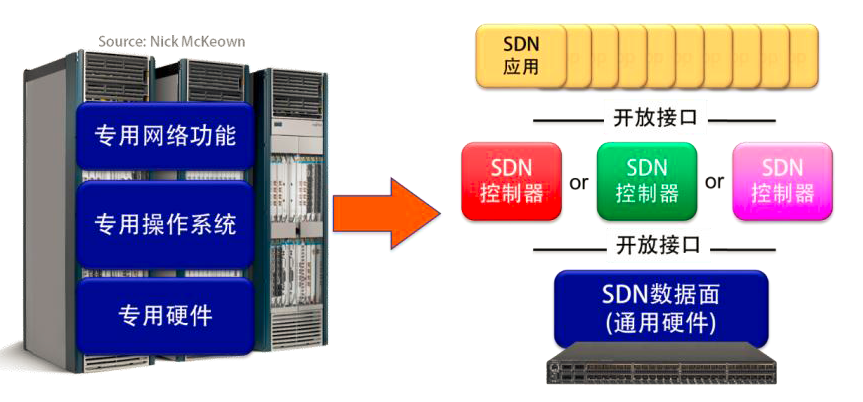
\includegraphics[width=4.0in]{figures/SchematicDiagram4EvolutionFromTraditionalNetworkArchitecture2SDNArchitecture}
  \caption{传统网络架构向SDN架构演进示意图}
  \label{fig:SchematicDiagram4EvolutionFromTraditionalNetworkArchitecture2SDNArchitecture}
\end{figure}



%有人认为,SDN就是OpenFlow;有人认为,SDN就是数控分离;还有人认为只要支持软件编程控制的网络就是SDN。 不同的人对SDN有着不一样的理解,正如一千个人眼中有一千个哈姆雷特。为探究SDN 的准确定义,我们将以ONF (Open Networking Foundation, 开放网络基金会)和ONRC (OpenFlow Network Research Center,开放网络研究中心) 对SDN的定义为切入点,深入探讨SDN的本质,一层一层揭开SDN 的神秘面纱,直到看清SDN的庐山真面目。ONRC 是SDN 创始人斯坦福大学教授Nick McKeown 和加州大学伯克利分校教授 Scott Shenker,以及大名鼎鼎的Larry Peterson教授共同同创建的研究架构。ONRC对SDN 的定义是:“SDN是一种逻辑集中控制的新网络架构,其关键属性包括:数据平面和控制平面分离;数据平面和控制平面之间有统一的开放接口OpenFlow。”在ONRC的定义中,SDN的特征表现为数据平面和控制平面分离,拥有逻辑集中式的控制平面,并通过统一而开放的南向接口来实现对网络的控制。ONRC强调了“数控分离”,逻辑集中式控制和统一、开放的接口。
%
%相比ONRC对SDN的定义,另一个重要的组织ONF对SDN定义做出了不同的描 述。ONF 是Nick McKeown 教授和Scott Shenker教授联合多家业界厂商发起的非营利性 开放组织,其工作的主要内容是推动SDN的标准化和商业化进程。ONF认为:“SDN 是一种支持动态、弹性管理的新型网络体系结构,是实现高带宽、动态网络的理想架构。 SDN将网络的控制平面和数据平面解耦分离,抽象了数据平面网络资源,并支持通过统 一的接口对网络直接进行编程控制”。相比之下,ONF 强调了 SDN对网络资源的抽象能 力和可编程能力。

%本质上,这两个组织给出的SDN定义并没有太大的差别,都强调了 SDN拥有数据 平面和控制平面解耦分离的特点,也都强调了 SDN支持通过软件编程对网络进行控制 的能力。但是ONRC更强调数控分离和集中控制等表现形式,而ONF则强调抽象和可 编程等功能。
%从ONRC和ONF对SDN的定义中可以了解到:

SDN不仅重构了网络的系统功能,实现了数控分离,也对网络资源进行了抽象,建立了新的网络抽象模型。SDN主要有如下三个特征:
\begin{enumerate}
  \item 网络开放可编程:SDN建立了新的网络抽象模型,为用户提供了一套完整的通用API,使用户可以在控制器上编程实现对网络的配置、管理和控制,从而加快网络业务部署的进程。
  \item 逻辑上的集中控制:主要是指对分布式网络状态的集中统一管理。在SDN架构中,控制器会担负起管理和收集所有网络状态信息的重任。逻辑集中控制为软件编程 定义网络功能提供了架构基础,也为网络自动化管理提供了可能。
  \item 数据平面与控制平面的分离:此处的分离是指数据平面与控制平面的解耦合。 数据平面和控制平面之间不再相互依赖,两者可以独立完成体系结构的演进,类似于计算机工业的intel模式,双方只需要遵循统一的开放接口进行通信即可。数 据平面与控制平面的分离是SDN架构区别于传统网络体系结构的重要标志,是网络获得更多可编程能力的架构基础。
\end{enumerate}

因此,只要符合以上三个特征的网络都可以称之为软件定义网络。在这三个特征中, 数据平面和控制平面分离为逻辑集中控制创造了条件,逻辑集中控制为开放可编程控制提供了架构基础,而网络开放可编程才是SDN的核心特征。
一般来说,SDN网络体系结构主要包括SDN网络应用、北向接口、SDN控制器、 南向接口和SDN 数据平面共五部分,如图\ref{fig:SDNArchitectureDiagram}所示。

\begin{figure}[htbp]
\centering
% Requires \usepackage{graphicx}
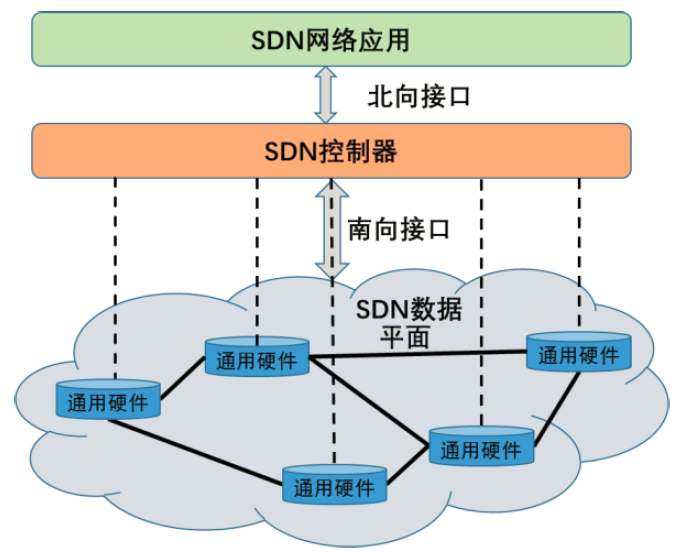
\includegraphics[width=4.0in]{figures/SDNArchitectureDiagram}
  \caption{SDN体系架构图}
  \label{fig:SDNArchitectureDiagram}
\end{figure}

现代电信网络提供多种高速通信,通过大规模的面向连接和分组交换的网络提供服务运行在光网络,数字用户线路(DSL),电缆连接甚至无线地面和卫星连接。因为社会很大程度上依赖于现代电信网络,已经做了很多工作来防止网络故障,例如,通过改善设备环境和材料的物理方面。然而,过去一个世纪的网络故障情形显示,高速骨干网络链路即使短暂的故障也会造成大量的数据包丢弃,严重影响通信质量。根据对Internet服务提供者(ISP)的观察,骨干网链路一年内大约有30\% 的概率会出现故障\cite{doerr2014all}。不论采取了哪些预防性保护措施,网络节点和链接将最终概率性的失灵并停止运作。链路故障是网络中较为普遍的现象。因此,加快故障的恢复速度,降低故障造成的业务丢弃已成为当前研究亟待解决的问题。

在面向连接的网络中,例如波长路由网络中,由于网络节点或链路的故障而造成的网络服务中断通常可以通过从源节点分配至少两个不相交的路径到每个网络连接的目的节点来防止中断\cite{kuipers2012overview}。然后监视从源节点到目标节点的连接状态,当网络连接的主路径故障失效时,可以重新配置连接以使用其备份路径继续保持工作。还可以同时在连接的主路径和备份路径上发送通信信息,因此不需要在主路径故障失效时进行重新配置。虽然找到从源节点到目的节点的一对(最小和)Min-Sum不相交路径是多项式可解的\cite{suurballe1974disjoint,suurballe1984quick},但由于存在陷阱拓扑\cite{dunn1994comparison},返回的路径可能远远大于节点之间的最短路径\cite{dunn1994comparison}。 另一种方法是找到一对Min-Min不相交的路径,其中主路径的权重最小化,而不是两条路径的权重之和(最小和),网络业务主要运行在主路径上,当出现故障时备份路径主要是保证业务非中断,而不一定保证原来主路径一样的服务质量,所以对主路径的权重代价尽量小,另外必须保证存在备份路径,但对于备份路径的权重不做严格的需求。然而Min-Min不相交路径问题是NP-hard\cite{guo2013finding}。

%在分组交换网络中,例如以太网或IP网络,没有连接状态,因为分组是通过在其所经过的每一个路由器上对报头进行本地检查而逐跳转发的。虽然在分组交换中使用不相交路径是可能通过端到端的动态检测监测方案(如双向转发检测(BFD)\cite{katz2010bidirectional}、以太网OAM/CFM\cite{mcfarland2005ethernet}或IP快速重路由\cite{shand2010ip}),然而该方法比面向连接的网络更加复杂。任何网络节点都可以在没有事先预约的情况下向任何其他网络节点发送消息,这也导致了O($|N|^2$)(其中$|N|$是网络节点的数目)对每个源/目的节点对可能被监视会话:与面向连接的网络相比,监视会话的数量被限制到O($|C|$)(其中$|C|$ 是实际连接的数量)。因此,在分组交换网络中,计算和维护所有可能的节点对的不相交路径可能是次优的。



在分组交换网络中,流量可以沿着主要路径的一部分重新路由,这在面向连接的网络中是不可能的。主路径上的每个中间节点在必要时具有通过另一个链路接口转发数据包的能力。此外,在分组经过故障重路由后,分组被定向到到达目的地的最短剩余路径,可能的方法是跟踪未受故障影响的(初始)主路径的其余部分。然而,配置全网配置需要复杂的转发规则构造,传统的分布式路由协议在计算和内存容量较低的嵌入式系统上难以实现。而新兴的软件定义的网络(SDN)方法可以促进这种网络功能的实现。

%SDN引入中央控制器可以监视网络的性能和功能,并在必要时重新编程。如果控制器可以像观察流量、丢包和延迟那样监测整个网络的健康状况\cite{van2014opennetmon},最基本的任务是保持节点之间的端到端连接。因此,当链路中断时,控制器需要重新配置网络以恢复或维护所有路径的端到端连接。然而,故障路径的恢复时间,除了检测时间外,还包括将事件通知控制器的传播时间所带来的延迟、路径重新计算以及控制器对网络的重新配置。因此,控制器启动的路径恢复可能需要超过100 ms才能完成,这是被认为太长的供应商网络,其中最多50 毫秒是可以容忍的\cite{niven2009requirements}。
在SDN控制器中,往往需要考虑在多约束下的路由问题\cite{akyildiz2014roadmap}。特别在业务发放的场景中,为了到达抗故障的效果,需要为业务寻找工作与保护两条路径。而且为了保证网络的通信质量,通常需要考虑时延,跳数,以及工作与保护路径间的分离约束。所以多约束下的路由问题对实 现网络资源实现高效快速调配和利用具有重要的意义。





\subsubsection{网络功能虚拟化NFV}
多样化的专有网络设备增加了服务提供商的资金和运营费用,同时也引起了网络僵化的问题。网络功能虚拟化(NFV)提出解决了这些问题,实现网络功能的纯软件商品通用的硬件。NFV 允许灵活的配置,部署和集中管理虚拟网络功能。结合SDN 软件定义NFV架构进一步提供灵活的流量操作和网络功能和资源的联合优化。这种体系结构有利于广泛的应用程序(例如服务链),并且正在成为NFV的主要形式。

目前的网络服务依赖于专有设备和不同的网络设备,这些设备是多种多样和专门创建的\cite{sherry2012making,wang2011untold,walfish2004middleboxes}。这种情况引发了所谓的网络僵化问题,阻碍了业务的增加和网络的升级。为了解决这一问题并减少资本支出和业务支出,虚拟化已成为一种将网络软件功能/应用程序与其支持的硬件分离的方法,并允许网络服务作为软件\cite{schaffrath2009network,chowdhury2010survey,chowdhury2009network} 加以实施。利用虚拟化技术,ETSI 工业规范组提出了网络功能虚拟化NFV,虚拟化以前的一些专有专用硬件执行的网络功能\cite{chiosi2012network,yue2013network},通过将网络功能与底层硬件设备分离,NFV在优化共享的物理基础设施之上提供了基于软件的网络功能的灵活配置。它通过利用低成本商品服务器来解决管理和控制这些封闭和专有设备的运营成本问题。

另一方面,随着软件定义网络SDN的发展,随着网络体系结构\cite{manzalini2014software,yeganeh2013scalability,ge20145g}的引入,将SDN 与NFV(软件定义的NFV体系结构)集成以实现各种网络控制和管理目标的趋势得到了明显的发展。当将SDN应用于NFV 时,可以帮助应对动态的挑战,资源管理,智能服务编排和故障恢复。通过SDN/NFV可以动态地为特定类型的服务链创建虚拟服务环境,从而避免了专用硬件和复杂的工作来提供新的服务请求。在使用SDN 的同时,NFV进一步实现了实时动态功能配置和灵活的业务转发。

软件定义的NFV利用网络虚拟化和逻辑上集中的智能来最大限度地减少服务提供成本,并最大限度地利用网络资源。在这种情况下,所获得的更高的资源利用率将对硬件设备引入较少的调查,这一方面简化了联网操作。此外,通过自动化当前手动密集的网络配置、部署和管理,显著减少了时间和操作复杂性,并且显著降低了手动错误,这提供了更好的可扩展性。另一方面,特别是在大型网络中,部署和提供新的服务通常导致需要长周期的验证、证明和长期和重复的测试过程。通过自动化NFV相关基础设施的控制、管理和协调,将显著缩短用于这些新服务的网络配置和操作变更的部署时间和操作成本。

服务链是软件定义的NFV能够发挥重要作用的主要领域\cite{friis2009service,lemmens2007enhancing}。在当前网络,一种服务链包括一套硬件专用网络设备,提供负载平衡器、防火墙、深度数据包检测(DPI)、 入侵检测系统(IDS)等服务,以支持专用的网络处理和应用\cite{greenberg2005clean,tschudin2001selnet,joseph2008policy,santos2008bridging}。 当涉及到新的服务需求时,新硬件设备必须通过某种顺序进行部署、安装和连接,这是非常耗时、复杂、高成本和容易出错的。这种网络服务的提供需要专门的计划为网络的变化和中断,另一方面,这会导致很高的资本支出和业务支出。当许多不同类型的服务序列被运营商专用于不同的业务流时,这种情况就会更加严重。另一方面,软件定义的NFV 体系结构可以简化服务链的部署和配置。它使在局域网、企业网络、数据中心和Interent 服务提供商网络中提供更容易和更便宜的服务。




为了获得当前和未来云计算的成功,网络虚拟化也是其中的关键,而SDN是网络可编程性的关键,SDN 由于其集中控制的特性,它最适合的领域应该是数据 中心中网络虚拟化的应用。SDN 要求集中控制,网络虚拟化也同样要求集中化控制,网络虚拟化可以为数据中心的每个“租户”提供自己的网络拓扑并控制其流量, 这种特性使得两者很自然地结合到一起了。SDN 可以在控制器应用和交换机转发 表之间提供标准接口,因此,是网络虚拟化的自然平台。然而,支持具有不同拓 扑和控制器应用的许多租户提出了可扩展的挑战性,所以SDN虚拟网络的概念应运而生,其中,虚拟网络服务是SDN 虚拟网络的一部分,也是部署防火墙、均衡 负载、网络路由和虚拟专用网(Virtual private network, VPN) 等按需求提供功能的 应用软件。在软件中,虚拟化网络服务消除了对昂贵的物理、专有和固定网络的 需要,这些设备都缺乏数据中心所需的灵活性和可扩展性。并且,现在的云计算 技术大大减缓了创建新网络服务的压力,同时,诸如网络创新的全球实验环境可 以让研究人员在共享基础设施的分片上进行大规模的实验,让租户共享物理资源, 虚拟化技术势必成为了这些基础架构中的关键。

%在网络虚拟化技术 中,一般认为网络虚拟化是使得多个逻辑网络共享一个物理网络,不过网络设计 中原有的层次结构不会被破坏,同样不被破坏保留的还有网络中的数据通道以及 所能提供的服务,所有这些特点都会让用户感觉自己在独享物理网络。


网络虚拟化\cite{chowdhury2009network}技术通过对物理网络络资源进行抽象、隔离和分配,可支持多个虚拟网络(Virtual Network, VN)共存于同一物理网络中。虚拟网络映射\cite{fischer2013virtual}(Virtual Network Embedding, VNE)是实现网络虚拟化的关键,旨在研究如何合理地将租户定制的虚拟网络请求(Virtual Network Request,VNR)映射到底层物理网络 (SubstrateNetwork, SN) 中,获取满足虚拟网络服务所需的物理网络资源,从而提高虚拟网络请求接受率和网络资源利用率。对于不同的虚拟网络和物理网拓扑,设计不同的映射
算法,会得到不同效率的映射方案,如何映射以确保网络资源的高效利用以及网
络的负载均衡,也是现在和未来网络研究的方向。在虚拟网络映射算法中,默认分配给租户的虚拟网络服务可以一直正常运行,但现实中,由于设备自身或者环境等问题有时会引发物理网络故障,进而影响租户的虚拟网络服务的可生存性。因此,为向租户提供一个高可生存的虚拟网络服务,一些研究者提出了多种可生存性虚拟网络映射算法\cite{herker2013survey}。

可生存性虚拟网络映射主要研究节点故障、链路故障或者同时考虑这两种故障的情况。在物理网络中,节点故障对于虚拟网络可用性的影响更大,所以本文将研究基于物理节点故障的可生存性虚拟网络映射(Survivable Virtual Network Embedding, SVNE)算法。


\subsection{课题研究目的和意义}
\textbf{SRLG分离路径的意义}

存储器和服务器的虚拟化带来了网络规模的增大和网络服务流畅性的提高,从而进一步加大了对自动化、多租户和多路径要的求迫切性,也带来了网络虚拟化的需求。虚拟化的主要思想就是要创建一个运行在被抽象的实际物理实体之上的更高层次的抽象。网络虚拟化出现,网络管理员不仅可以随时随地选择创建网络,还能够任意扩展和收缩已经存在的网络。智能的虚拟化软件在完成这些任务时,位于上层的虚拟网络不需要知道底层物理拓扑或者配置发生了什么变化,上层虚拟网络在向底层虚拟网络映射时,为了达到低成本高收益的效果,需要找到最有效的嵌入算法。

而由于SDN的集中控制性能,相比传统的分布式算法,集中控制器可以更好地执行最优路径的计算和提供特殊服务需求,这是因为:
\begin{itemize}
  \item 可以考虑更 多的因素,包括当前带宽的负载情况等
  \item 有一个更稳定的网络全局视图
  \item 可以在服务器性能较高的内存和处 理器上执行计算,而不是在网络设备能力有限的可用内存和处理器上执行
\end{itemize}


为了支持具有不同拓扑结构的虚拟网络,需要一种嵌入方法将虚拟网络映射 到物理设施,并将物理网故障如链路或交换机故障映射到虚拟网络组件,任何虚 拟化解决方案都必须快速执行这些映射操作,以便每个租户可以对其虚拟网络提 供实时控制。在将虚拟网络映射到物理网络时,嵌入算法是其中的关键,在将虚 拟网络的节点和链路进行映射时,需要找到最佳路由完成资源的配置,现有的路由算法己经很多,对于不同的应用场景,很难评判算法性能的好坏,较好的解决 办法是针对不同的应用场景设计满足要求的算法,使算法的性能和效率能够优化。 另外,在虚拟网络的映射过程中,为了防止底层物理资源出现故障失效的情况, 可以从用户层面和网络层面进行可生存性的研究。


